\documentclass{beamer}
\usepackage{config_beamer} 

\title{Introduction to Quantitative Methods}
\subtitle{(Master 1 EEI)}
\author{Maxime Chabriel}
\date{2024-2025}

\begin{document}

\maketitle

\section{General Introduction}
\begin{frame}{Who I am/What I do}
    \begin{itemize}
        \item PhD student in Economic history at ENS de Lyon (CERGIC)
        \vspace{0.4cm}
        \item ENSAE + Master in International Development (ScPo)
        \vspace{0.4cm}
        \item \textbf{Contact:}
        \vspace{0.2cm}
        \begin{itemize}
            \item Office: D4-tbd
        \vspace{0.2cm}
            \item Mail: maxime.chabriel@proton.me
        \end{itemize}
    \end{itemize}
\end{frame}


\subsection{Organization of the Course}
\begin{frame}{Global Organization}
    \begin{itemize}
        \item 12 $\times$ 2h class, every Thursdays
        \vspace{0.3cm}
        \item Discover/Recall the basic quantitative tools used in social and political sciences
        \vspace{0.3cm}
        \item Provide \textbf{intuition} on how to deal with quantitative data, and we will cover a few ways to infer results from it
        \vspace{0.3cm}
        \item \textbf{Preparation course}, so no strict curriculum
        \\ $\rightarrow$ The main objective is to adapt to your needs
    \end{itemize}
\end{frame}


\begin{frame}{Global Outline}
    \begin{enumerate}
        \item General Introduction and Conceptual Tools (2h)
        \vspace{0.3cm}
        \item Univariate Analysis and Descriptive Statistics (6h)
        \vspace{0.3cm}
        \item Multivariate Analysis (6h)
        \vspace{0.3cm}
        \item Introduction to linear regressions and causal analysis (4h)
        \vspace{0.3cm}
        \item Introduction to R (4h)
        \vspace{0.3cm}
        \item Final written exam (2h) 
    \end{itemize}
\end{frame}

\begin{frame}{Evaluation}
    \begin{itemize}
        \item Continuous assessment (20\%)
        \vspace{0.2cm}
        \item A 5-10 pages at home report on a chosen topic (40\%) \\
        I will give the instructions at the end of the Univariate analysis section
        \vspace{0.2cm}
        \item A final written theoretical exam (40\%)
    \end{itemize}
\end{frame}

\section{Survey time!}
\begin{frame}[plain]
    \centering \Large
    \textbf{Survey time!}
\end{frame}

\section{What are Quantitative Methods?}
\begin{frame}[plain]
    \centering \Large
    \textbf{What are Quantitative Methods?}
\end{frame}

\begin{frame}
    \begin{itemize}
        \item Measuring
        \begin{itemize}
            \item surveys, lexicometry, accounting...
            \item building indicators (GDP, HDI, debt ratio...)
        \end{itemize}
        \vspace{0.2cm}
        \item Creating statistics
        \begin{itemize}
            \item mean, median, quantile...
        \end{itemize}
        \vspace{0.2cm}
        \item Regression analysis (causal inference, effect size)
        \vspace{0.2cm}
        \item Machine Learning (clustering, prediction, natural language processing)
    \end{itemize}
\end{frame}

\section{Why use Quantitative Methods?}
\begin{frame}[plain]
    \centering \Large
    \textbf{Why use Quantitative Methods?}
\end{frame}

\begin{frame}{Pros and Cons of Quantitative Methods}
    \textbf{Pros:}
    \begin{itemize}
        \item Synthesis power
        \item More "formal" and persuasive (especially visually)
        \item Data can help to look at the big picture
        \item We can use mathematical theory to build  confidence intervals, causal inference etc...
    \end{itemize}
    \vspace{0.2cm}
    \textbf{Cons:}
    \begin{itemize}
        \item Not everything can be (relevantly) quantified
        \item May lack nuance or context
        \item We cannot ignore the production process of the data (a database is a social construct)
    \end{itemize}
\end{frame}

\begin{frame}
    \begin{itemize}
        \item $\rightarrow$ In social sciences, one cannot rely only on quantitative or qualitative data, but needs to make both sources dialogue
        \vspace{0.2cm}
        \item In practice, the quantitative and qualitative methods of today are so advanced that no researcher is specialised in both
        \vspace{0.2cm}
        \item $\rightarrow$ There are communication issues! Or even conflicts, as results can clash
        \vspace{0.2cm}
        \item Famous recent example : \textit{Peut-on faire l’économie de l’histoire ? Verdun, Vichy, et les conditions d’un dialogue entre disciplines} 2021\\
        https://devhist.hypotheses.org/3921 
        \vspace{0.2cm}
        \item Hence the necessity to be literate in both methods
    \end{itemize}
\end{frame}

\section{The necessary steps of a good quantitative analysis}
\begin{frame}[plain]
    \centering \Large
    \textbf{The necessary steps of a good quantitative analysis}
\end{frame}

\begin{frame}
    \begin{itemize}
        \item \textbf{Define} your research question / the purpose of your analysis
        \begin{itemize}
            \item Check the literature. Has your question been answered somewhere else? If so, were you convinced by their method?
            \item Do you really need to do a quantitative analysis?
        \end{itemize}
        \item \textbf{Choose} your data
        \begin{itemize}
            \item Compare the sources
            \item Compare the details/reliability of their documentations
        \end{itemize}
        \item \textbf{Explore, Know} your dataset, describe its variables
        \begin{itemize}
            \item Is your data incoherent? Are there missing values?
            \item New variables / peculiar observations can give you new ideas
        \end{itemize}
        \item \textbf{Choose} your method of analysis.
        \begin{itemize}
            \item Visualisations? 
            \item Indicators to build?
            \item Causal model?
        \end{itemize}
        \item \textbf{Robustness checks}
        \begin{itemize}
            \item Everything you (or someone else) could have done differently, do it and compare your results
        \end{itemize}
    \end{itemize}
\end{frame}

\section{Good practices}
\begin{frame}[plain]
    \centering \Large
    \textbf{Good practices}
\end{frame}

\begin{frame}
    \begin{itemize}
        \item Along the way, take good notes of your data source, results, choices etc.
        \vspace{0.2cm}
        \item Take some time cleaning and formatting your data
        \vspace{0.2cm}
        \item This includes choosing intelligent file names and folder structure
        \vspace{0.2cm}
        \item Save frequently!
        \vspace{0.2cm}
        \item Do not hesitate to test things
        \vspace{0.2cm}
        \item Be honest. If some results do not go your way, do not hide it and find possible explanations
    \end{itemize}
\end{frame}

\section{Definitions}
\begin{frame}[plain]
    \centering \Large
    \textbf{Definitions}
\end{frame}

\begin{frame}
    \begin{itemize}
        \item \textbf{Population} : The group of individuals / objects / events of which we want to know some characteristics or implement an analysis.
        \vspace{0.2cm}
        \item \textbf{Sample} : The subset of the population on which information has been gathered.
        \vspace{0.2cm}
        \item \textbf{Observation} : One unit of the sample.
        \vspace{0.2cm}
        \item \textbf{Variable} : A characteristic of the population that has been measured on the sample. 
        \vspace{0.2cm}
        \item \textbf{Sample representativity / Sample bias} : The extent to which the sample represents / does not represent the population.
        \vspace{0.2cm}
        \item \textbf{Dataframe / Dataset} : Computer object used to store the variables and the observations.
    \end{itemize}
\end{frame}

\begin{frame}
    Wooclap : wooclap.com + event code PTHGYF
    \begin{itemize}
        \item \textbf{Population ?} :
    \end{itemize}
\end{frame}

\begin{frame}{Dataset example}
    \begin{figure}
        \centering
        \caption{Screenshot from Rstudio}
        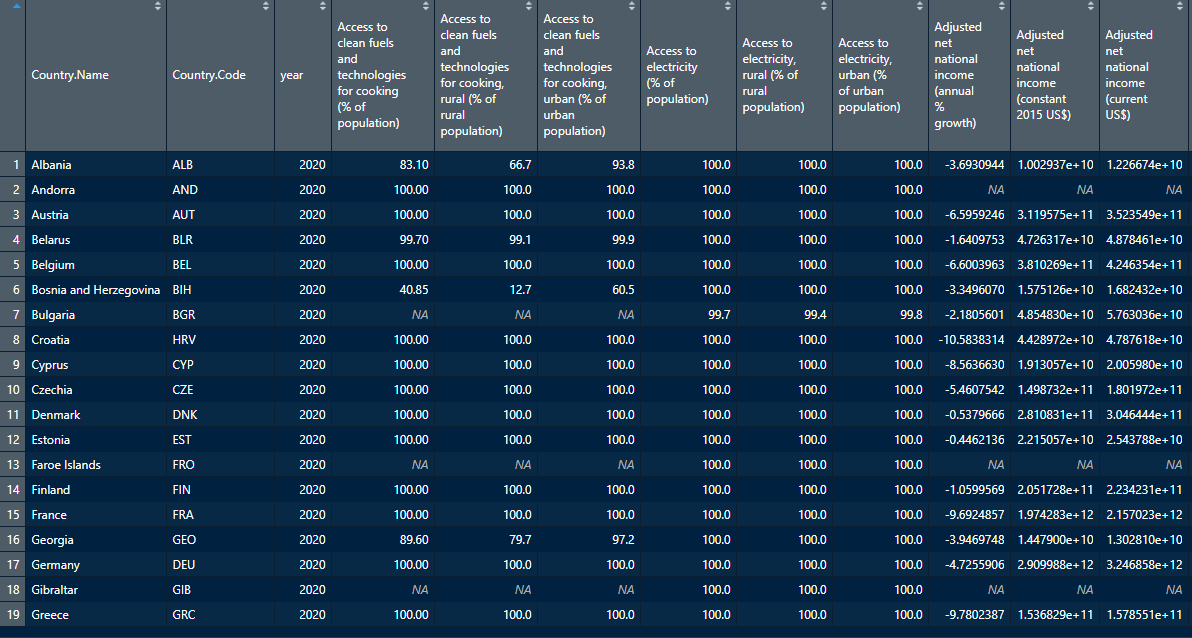
\includegraphics[scale=0.3]{Picture/Data Structure 2.png}
        \caption*{\textit{\raggedright \tiny Data extracted from the World Bank's World Development Indicators}}
    \end{figure}
\end{frame}

\begin{frame}
    \begin{itemize}
        \item \textbf{Population} : Countries
        \vspace{0.2cm}
        \item \textbf{Sample ?} : 
    \end{itemize}
\end{frame}

\begin{frame}{Dataset example}
    \begin{figure}
        \centering
        \caption{Screenshot from Rstudio}
        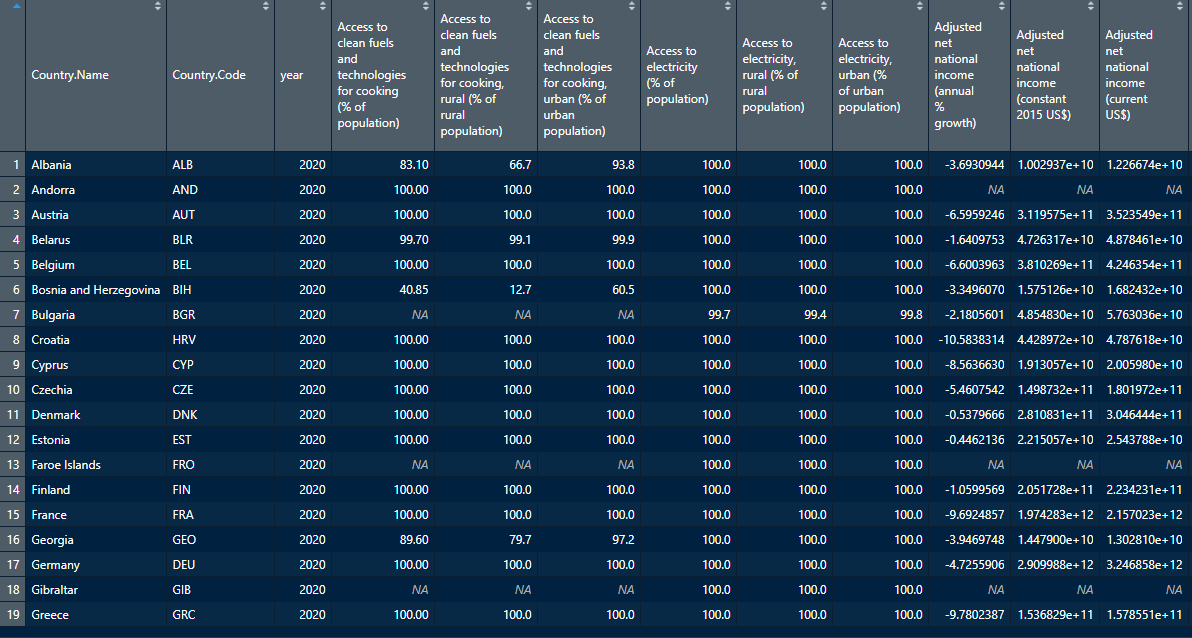
\includegraphics[scale=0.3]{Picture/Data Structure 2.png}
        \caption*{\textit{\raggedright \tiny Data extracted from the World Bank's World Development Indicators}}
    \end{figure}
\end{frame}

\begin{frame}
    \begin{itemize}
        \item \textbf{Population} : Countries
        \vspace{0.2cm}
        \item \textbf{Sample} : European Countries
        \vspace{0.2cm}
        \item \textbf{Observation ?} : 
        \vspace{0.2cm}
        \item \textbf{Variable ?} : 
        \vspace{0.2cm}
    \end{itemize}
\end{frame}

\begin{frame}{Dataset example}
    \begin{figure}
        \centering
        \caption{Screenshot from Rstudio}
        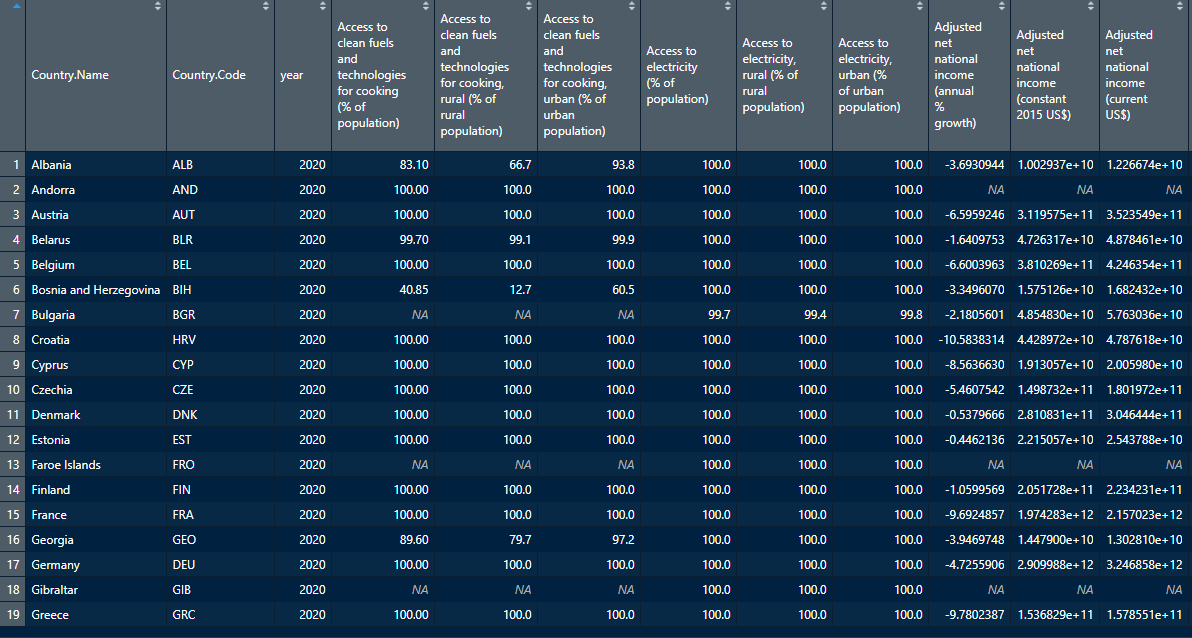
\includegraphics[scale=0.3]{Picture/Data Structure 2.png}
        \caption*{\textit{\raggedright \tiny Data extracted from the World Bank's World Development Indicators}}
    \end{figure}
\end{frame}

\begin{frame}
    \begin{itemize}
        \item \textbf{Population} : Countries
        \vspace{0.2cm}
        \item \textbf{Sample} : European Countries
        \vspace{0.2cm}
        \item \textbf{Observation} : One line of the dataframe
        \vspace{0.2cm}
        \item \textbf{Variable} : One column of the dataframe
        \vspace{0.2cm}
        \item \textbf{Sample representativity / Sample bias ?} :
    \end{itemize}
\end{frame}

\begin{frame}{Dataset example}
    \begin{figure}
        \centering
        \caption{Screenshot from Rstudio}
        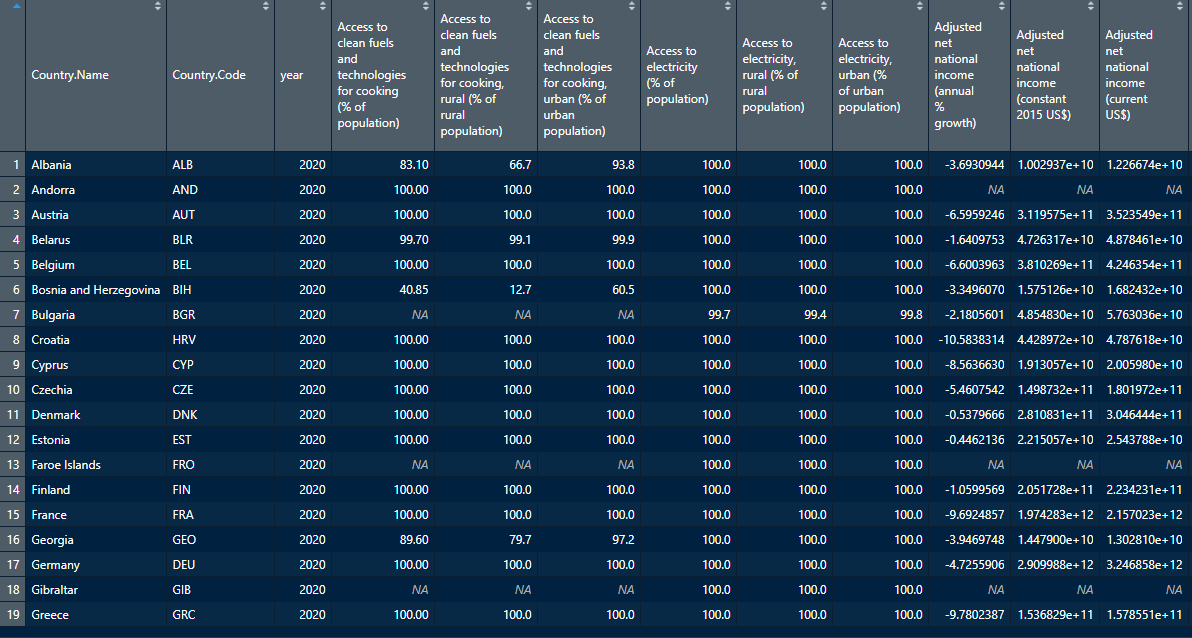
\includegraphics[scale=0.3]{Picture/Data Structure 2.png}
        \caption*{\textit{\raggedright \tiny Data extracted from the World Bank's World Development Indicators}}
    \end{figure}
\end{frame}

\begin{frame}
    \begin{itemize}
        \item \textbf{Population} : Countries
        \vspace{0.2cm}
        \item \textbf{Sample} : European Countries
        \vspace{0.2cm}
        \item \textbf{Observation} : One line of the dataframe
        \vspace{0.2cm}
        \item \textbf{Variable} : One column of the dataframe
        \vspace{0.2cm}
        \item \textbf{Sample representativity / Sample bias} : Mostly rich/developped countries
        \vspace{0.2cm}
        \item \textbf{Dataframe / Dataset} : World Development Indicators \\
        https://datacatalog.worldbank.org/search/dataset/0037712/World-Development-Indicators
    \end{itemize}
\end{frame}

\begin{frame}
    \textbf{Variable types}
    \vspace{0.2cm}
    \begin{itemize}
        \item \textbf{Qualitative variable} : A variable that cannot be represented by a number
        \begin{itemize}
            \item \textbf{Nominal categorical variable} (continent, dominant religion, currency, political regime)
            \item \textbf{Ordinal categorical variable} : When categories can be hierarchised
        \end{itemize}
    \end{itemize}
\end{frame}

\begin{frame}
    \textbf{Variable types}
    \vspace{0.2cm}
    \begin{itemize}
        \item \textbf{Qualitative variable} : A variable that cannot be represented by a number
        \begin{itemize}
            \item \textbf{Nominal categorical variable} (continent, dominant religion, currency, political regime)
            \item \textbf{Ordinal categorical variable} : When categories can be hierarchised (income level, political regime)
        \end{itemize}
        \vspace{0.2cm}
        \item \textbf{Quantitative variable}
        \begin{itemize}
            \item \textbf{Discrete variable} (rank, number of neighbors, year)
            \item \textbf{Continuous variable} (income, land size, time)
        \end{itemize}
    \end{itemize}
\end{frame}

\begin{frame}
    \textbf{Variable types}
    \vspace{0.2cm}
    \begin{itemize}
        \item \textbf{Qualitative variable} : A variable that is not represented by numeric values
        \begin{itemize}
            \item \textbf{Nominal categorical variable} (continent, dominant religion, currency, political regime)
            \item \textbf{Ordinal categorical variable} : When categories are hierarchised (income level, political regime)
        \end{itemize}
        \item \textbf{Quantitative variable}
        \begin{itemize}
            \item \textbf{Discrete variable} (rank, number of neighbors, year)
            \item \textbf{Continuous variable} (income, land size, time, population(!))
            \item \textbf{NB} Any Quantitative variable can be converted to an Ordinal categorical variable using intervals (ex: income levels)
        \end{itemize}
        \item \textbf{Other} :
        \begin{itemize}
            \item \textbf{Dummy / Boolean} : Takes the value 1 or 0 to decompose categorical variables. Or to code yes/no questions (landlocked, free elections, war)
            \item \textbf{Mixed} (year of decolonisation, age of elected leader). Also, some people like to encode their missing values with the numbers -1 or 99
        \end{itemize}
    \end{itemize}
\end{frame}

\end{document}
